\documentclass[tikz,border=4pt]{standalone}
% Paleta y fuentes compartidas por el libro y las figuras (única fuente de verdad).
\RequirePackage{xcolor}
\definecolor{oxido}{HTML}{B7410E}
\definecolor{cobre}{HTML}{D27D2D}
\definecolor{carbon}{HTML}{2B2B2B}
\definecolor{azul}{HTML}{1F5F8B}
\definecolor{arena}{HTML}{F4EDE4}

\usepackage{fontspec}
\setsansfont{FiraSans}[Extension=.otf,UprightFont=*-Regular,BoldFont=*-SemiBold,ItalicFont=*-Italic,BoldItalicFont=*-SemiBoldItalic]
\setmonofont{FiraMono}[Extension=.otf,UprightFont=*-Regular,BoldFont=*-Medium,Scale=0.95]
\usetikzlibrary{arrows.meta,calc,positioning}
\begin{document}
\sffamily\small
% Línea de tiempo vertical 2025--2026: fecha a la izquierda, hito a la derecha.
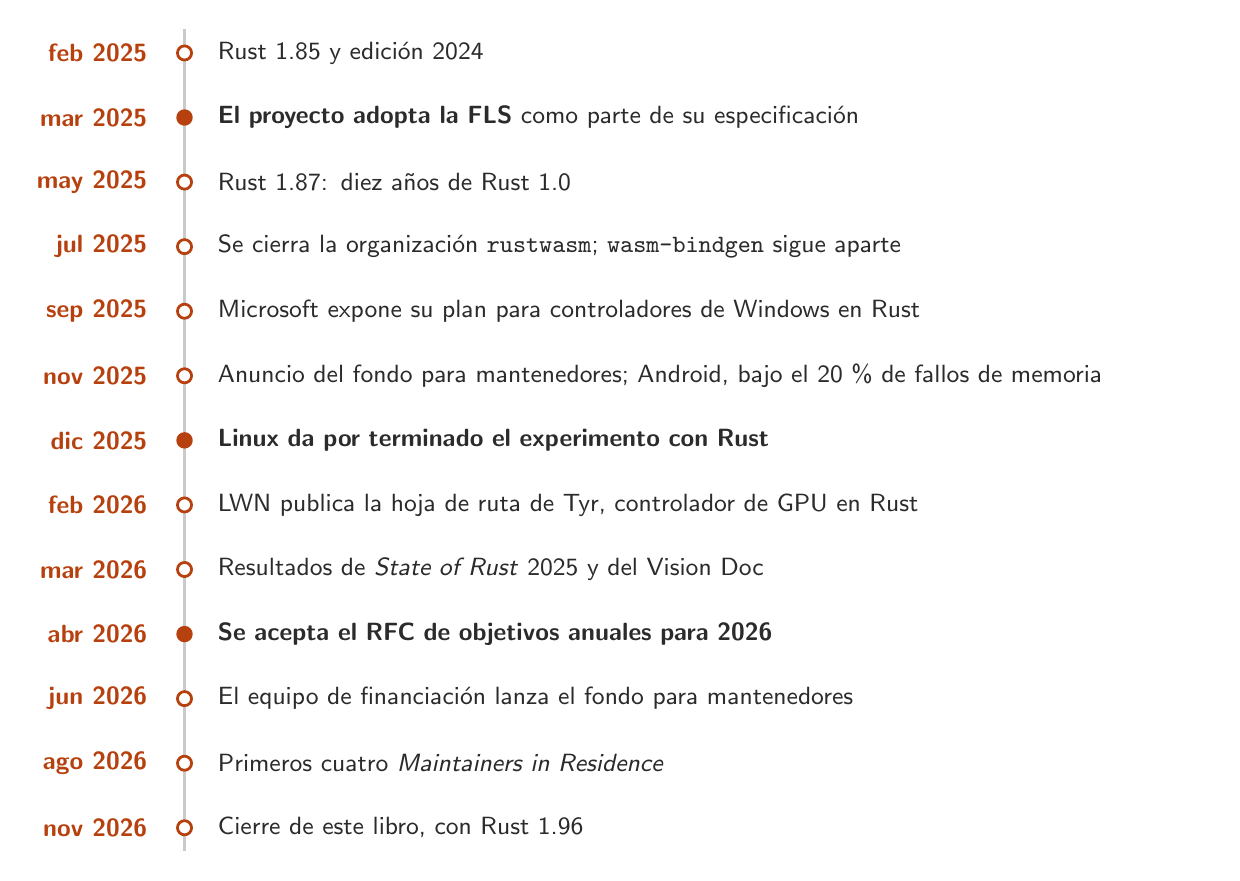
\begin{tikzpicture}[
  fecha/.style={font=\sffamily\bfseries\small,text=oxido,anchor=east},
  hito/.style={font=\sffamily\small,text=carbon,anchor=west,text width=125mm,align=left},
  punto/.style={circle,fill=oxido,inner sep=2.1pt},
  claro/.style={circle,draw=oxido,fill=white,line width=1pt,inner sep=1.8pt}]
  \def\paso{0.82}
  \draw[carbon!25,line width=1.2pt] (0,0.3) -- (0,-12*\paso-0.3);
  \foreach \a/\t/\e [count=\i from 0] in {
    feb 2025/{Rust 1.85 y edición 2024}/claro,
    mar 2025/{\textbf{El proyecto adopta la FLS} como parte de su especificación}/punto,
    may 2025/{Rust 1.87: diez años de Rust 1.0}/claro,
    jul 2025/{Se cierra la organización \texttt{rustwasm}; \texttt{wasm-bindgen} sigue aparte}/claro,
    sep 2025/{Microsoft expone su plan para controladores de Windows en Rust}/claro,
    nov 2025/{Anuncio del fondo para mantenedores; Android, bajo el 20~\% de fallos de memoria}/claro,
    dic 2025/{\textbf{Linux da por terminado el experimento con Rust}}/punto,
    feb 2026/{LWN publica la hoja de ruta de Tyr, controlador de GPU en Rust}/claro,
    mar 2026/{Resultados de \emph{State of Rust} 2025 y del Vision Doc}/claro,
    abr 2026/{\textbf{Se acepta el RFC de objetivos anuales para 2026}}/punto,
    jun 2026/{El equipo de financiación lanza el fondo para mantenedores}/claro,
    ago 2026/{Primeros cuatro \emph{Maintainers in Residence}}/claro,
    nov 2026/{Cierre de este libro, con Rust 1.96}/claro}
  {
    \node[\e] at (0,-\i*\paso) {};
    \node[fecha] at (-0.35,-\i*\paso) {\a};
    \node[hito] at (0.3,-\i*\paso) {\hyphenpenalty=10000 \t};
  }
\end{tikzpicture}
\end{document}
